\documentclass[12pt]{article}
\usepackage[margin=1in]{geometry}
\usepackage{amsmath,amssymb,amsthm,booktabs,graphicx,natbib,microtype}
\newtheorem{theorem}{Theorem}
\newtheorem{proposition}[theorem]{Proposition}
\newtheorem{corollary}[theorem]{Corollary}
\newtheorem{remark}[theorem]{Remark}
\title{Spectral-Reset Cross-Action Cancellation\\\large An Exact Tail-Coupling Identity and a Four-Mode Bridge Obstruction}
\author{Prime Dynamics Theory Program}
\date{July 2026}

\begin{document}
\maketitle

\begin{abstract}
RH-156 closes a finite native reset support floor, but the earlier
directional architecture uses a different object: the projected recent cross
$(I-P)RP$.  We determine whether a contemporaneous full-memory spectral reset
can bridge the two constructions.

Let $M=R+T$ and let $P$ be a spectral projector of $M$.  Spectral invariance
gives the exact cancellation
\[
 (I-P)RP=-(I-P)TP.
\]
Thus the recent projected cross sees only old-tail coupling.  A positive and
well-conditioned native compression $PRP$ supplies no positive lower for any
cross singular value; the obstruction remains even when $\|T\|$ is fixed and
nonzero, because $T$ may commute with $P$.

We derive an outward perturbation radius for
$J(P,T)=(I-P)TP$.  The frozen tail is exactly
$T_t=\eta^dM_{t-d}$, so its matrix radius is inherited from RH-151.  Fifty of
130 snapshots have inactive tail and therefore exact zero cross action.  Of
the 80 active snapshots, only 54 certify a positive fourth coupling singular
value; 26 hit the packet/tail radius wall.  The RH-154 terminal half certifies
only 30 of 62 snapshots, and only two of ten terminal snapshots have four
certified modes.  Hence the native support cannot be identified directly
with the old projected-cross support.  A lagged or hybrid reset packet is the
next controlled alternative.
\end{abstract}

\section{Two support objects that need not agree}
The native pair uses $PRP$ and $PTP$ inside the selected packet.  The older
directional route instead starts from the off-diagonal action
\[
 K_R=(I-P)RP,
\]
selects four right singular directions, and builds a wedge/capacity support
from their images.  Positivity of $PRP$ does not normally imply that $K_R$
has any rank.  For a spectral reset the relation is even more rigid.

\section{Exact cross-action cancellation}
\begin{theorem}[Spectral-reset cancellation]\label{thm:cancel}
Let $M=R+T$ be Hermitian and let $P$ be any spectral projector of $M$.  Then
\[
 (I-P)RP=-(I-P)TP.
\]
Consequently
\[
 \sigma_k((I-P)RP)=\sigma_k((I-P)TP)\leq\|T\|
\]
for every singular-value index $k$.
\end{theorem}
\begin{proof}
Spectral invariance gives $(I-P)MP=0$.  Substitute $M=R+T$ and rearrange.
The singular-value identity follows by multiplication by $-1$, and the upper
bound follows from contractivity of orthogonal projections.
\end{proof}

\begin{proposition}[No native-to-cross lower]\label{prop:none}
No positive lower for $\sigma_k((I-P)RP)$ follows from positive eigenvalue
endpoints for $PRP$, a positive overlap lower, and an upper or exact value of
$\|T\|$.  This remains true for every $k\geq1$.
\end{proposition}
\begin{proof}
Choose $R,T$, and $P$ diagonal in one common basis, with $PRP\succ0$ and
$\|T\|$ equal to any prescribed nonnegative value.  Then
$(I-P)TP=0$, so Theorem~\ref{thm:cancel} gives zero recent cross.  The native
Gram can simultaneously have arbitrary positive endpoint bounds.
\end{proof}

The missing datum is therefore explicit: a lower bound on the off-diagonal
tail coupling itself, such as
$\sigma_4((I-P)TP)\geq j_*>0$.  Tail mass alone points in the opposite
direction by supplying only an upper.

\section{Outward tail-coupling balls}
Let $Q$ be the exact reset projector, $P$ its center,
$\|Q-P\|\leq\epsilon$, and let the exact tail obey
$\|T-\widehat T\|\leq r_T$.

\begin{theorem}[Coupling perturbation radius]\label{thm:radius}
For $J(P,T)=(I-P)TP$,
\[
 \|J(Q,T)-J(P,\widehat T)\|
 \leq r_T+2\|\widehat T\|\epsilon.
\]
Hence each exact coupling singular value lies within this radius of its
nominal counterpart.
\end{theorem}
\begin{proof}
First change the tail at fixed $Q$, costing at most $r_T$.  At fixed
$\widehat T$, expand
\[
 J(Q,\widehat T)-J(P,\widehat T)
 =(P-Q)\widehat TQ+(I-P)\widehat T(Q-P).
\]
The two terms cost at most $\|\widehat T\|\epsilon$ each.  Singular-value
Weyl bounds finish the proof \citep{Bhatia1997,StewartSun1990}.
\end{proof}

For geometric memory at depth $d$,
\[
 T_t=\eta^dM_{t-d}\qquad(t\geq d).
\]
Therefore the archived RH-151 full-memory radius at time $t-d$, multiplied
by $\eta^d$, is already a tail radius.  No new source interval computation is
required.

\section{The 130-snapshot bridge audit}
At the fifty snapshots with $t<d=5$, the exact tail is zero.  Theorem
\ref{thm:cancel} makes the exact recent cross zero as well, regardless of the
strong native support floor.

The remaining eighty snapshots have active tail.  Applying
Theorem~\ref{thm:radius} to the fourth singular value certifies 54 positive
four-mode couplings and leaves 26 at zero lower.  Positive normalized
four-mode base lowers range from $3.2783\times10^{-4}$ to $0.57658$, with
median $0.02495$.  Their absolute fourth-singular lowers are tiny, from
$1.58\times10^{-20}$ to $5.53\times10^{-16}$, reflecting the
$\eta^5$ tail scale.

Only the two $\sigma=0.08$ channels certify every active snapshot.  At finer
scales the fourth-mode lower disappears near the terminal weak-gap region.
Only two of ten terminal snapshots certify four modes.  The delayed
terminal-half atlas contains 62 snapshots, six with exact zero tail and only
30 with positive fourth-coupling lower.  Delaying removes overlap births but
cannot repair spectral invariance.

\begin{figure}[t]
\centering
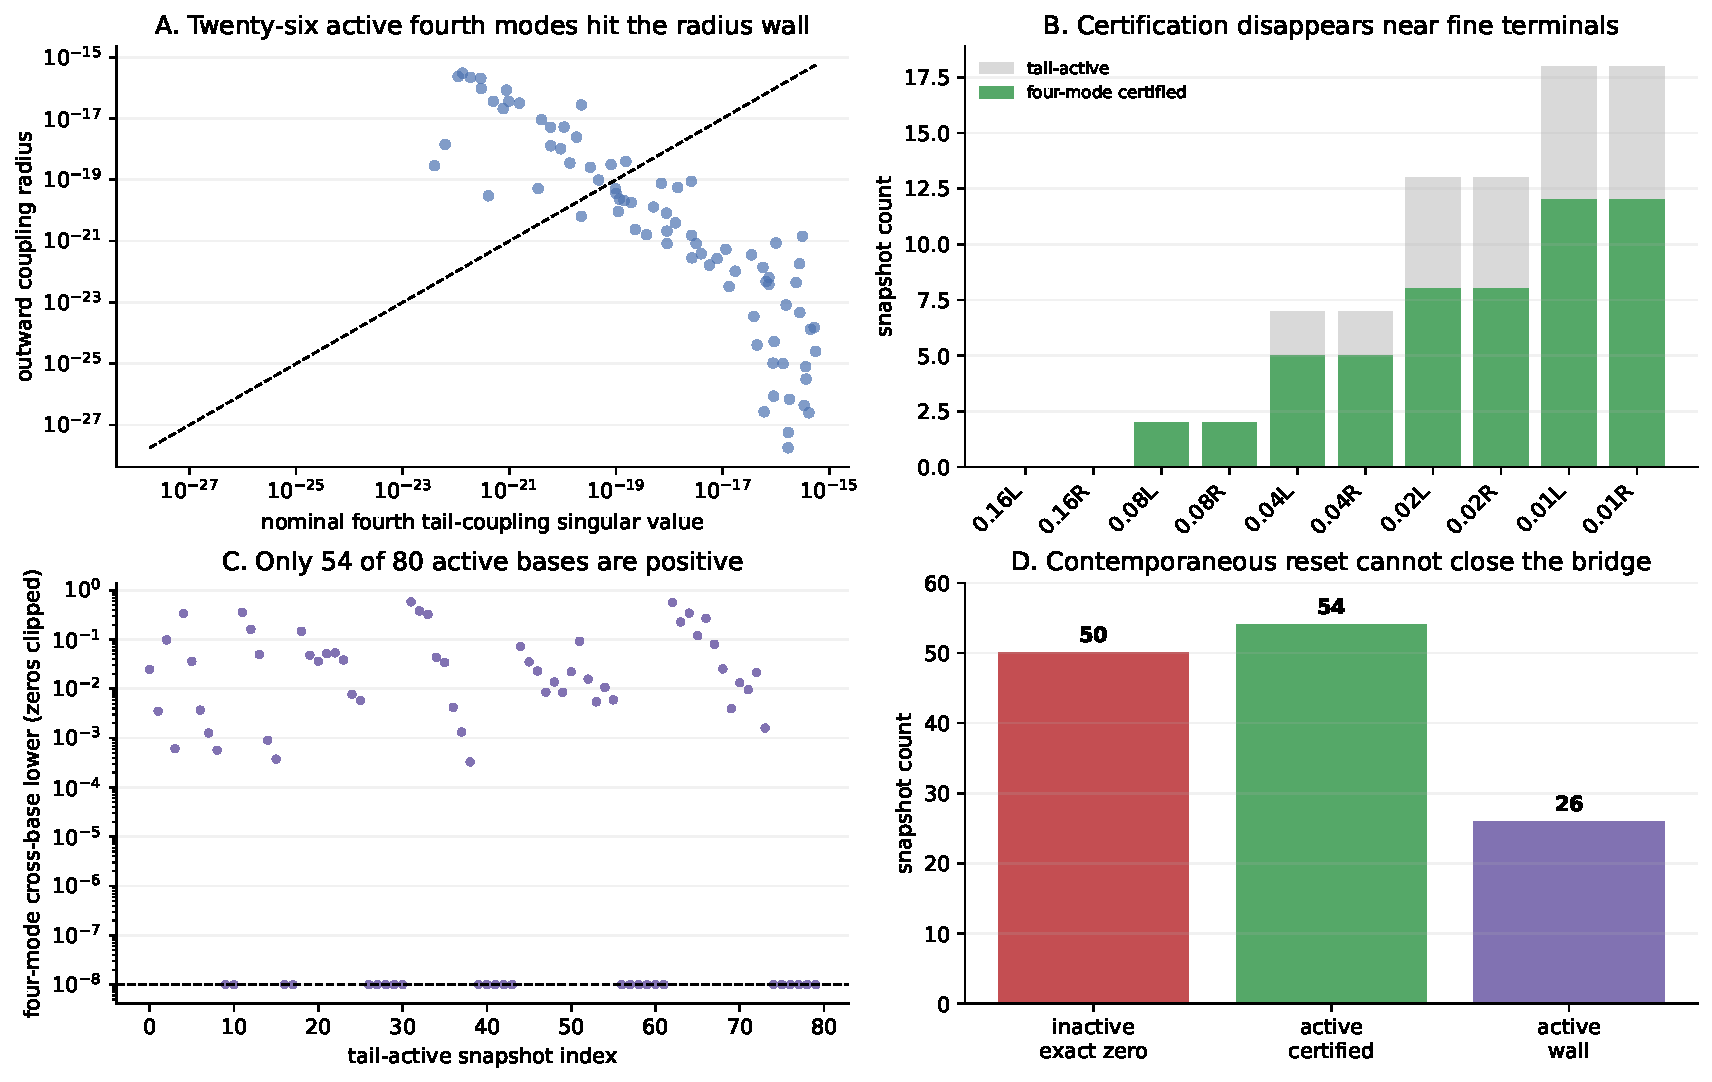
\includegraphics[width=\textwidth]{figures/spectral_reset_cross_action_cancellation.pdf}
\caption{Fourth-coupling radii, channel counts, positive normalized bases,
and the exact-zero/positive/wall decomposition.}
\label{fig:audit}
\end{figure}

\section{Route consequence and boundary}
RH-157 rejects one tempting identification without damaging RH-156.  The
native reset support is a valid finite functional, but the contemporaneous
spectral packet is deliberately invariant under the full memory; its
projected recent cross is therefore only a small tail leakage.  Forcing it
into the recursive directional architecture discards the main recent energy.

A lagged packet $P_{t-1}$ is not invariant under $M_t$ and may restore a
substantial cross while RH-152 controls its angle to $P_t$.  A hybrid between
$P_{t-1}$ and $P_t$ is another controlled option.  We have not proved either
bridge, an all-level four-coupling law, Stage A, a Hilbert--Polya operator,
zeta-zero identification, or the Riemann Hypothesis.

\bibliographystyle{plainnat}
\bibliography{references}
\end{document}
